

\documentclass{article}

\usepackage{tikz}
\usetikzlibrary{arrows,shapes,automata,petri,positioning,calc}
\tikzset{
    place/.style={
        rectangle,
        thick,
        draw=black,
        fill=gray!50,
        minimum size=6mm,
    },
}

\begin{document}


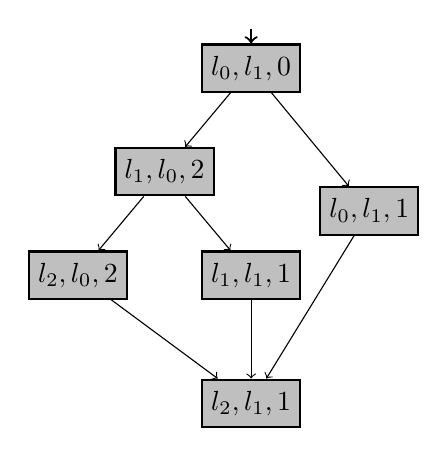
\begin{tikzpicture}

    % Nodes and position definitions
    \node [place] (N1) {$l_0,l_1,0$};
    \coordinate[node distance=1.1cm,left of=N1] (left-N1);
    \coordinate[node distance=1.5cm,right of=N1] (right-N1);
    \coordinate[node distance=0.5cm,above of=N1] (above-N1);

    \node [place] (S2) [below=of left-N1] {$l_1,l_0,2$};
    \coordinate[node distance=1.1cm,left of=S2] (left-S2);
    \coordinate[node distance=1.1cm,right of=S2] (right-S2);

    \node [place] (S3) [node distance=1.5cm,below =of right-N1] {$l_0,l_1,1$};    
    \coordinate[node distance=1.1cm,left of=S3] (left-S3);
    \coordinate[node distance=1.1cm,right of=S3] (right-S3);

    \node [place] (S4) [below=of left-S2] {$l_2,l_0,2$};
    \coordinate[node distance=1.1cm,left of=S4] (left-S4);
    \coordinate[node distance=1.1cm,right of=S4] (right-S4);

    \node [place] (S5) [below=of right-S2] {$l_1,l_1,1$};
    \coordinate[node distance=1.1cm,left of=S5] (left-S5);
    \coordinate[node distance=1.1cm,right of=S5] (right-S5);

    \node [place] (S6) [below=of S5]  {$l_2,l_1,1$};

    % Vertex definitions
    \draw[->, thick] (above-N1) -- (N1);
    \path[->] (N1) edge node {} (S2);
    \path[->] (N1) edge node {} (S3);
    \path[->] (S2) edge node {} (S4);
    \path[->] (S2) edge node {} (S5);
    \path[->] (S4) edge node {} (S6);
    \path[->] (S5) edge node {} (S6);
    \path[->] (S3) edge node {} (S6);
\end{tikzpicture}
\end{document}
